\documentclass{article}
\usepackage[margin=0.75in]{geometry}
\usepackage{enumitem}
\usepackage{setspace}
\usepackage{amsmath}
\usepackage{amssymb}
\usepackage{physics}
\usepackage{relsize}
\usepackage{graphicx}

\title{CS 143 Homework 6}
\date{3/9/2021}
\author{Jiaping Zeng}

\begin{document}
\setstretch{1.35}
\maketitle

\begin{enumerate}
    \item \begin{enumerate}
              \item $ $
                    \begin{center}
                        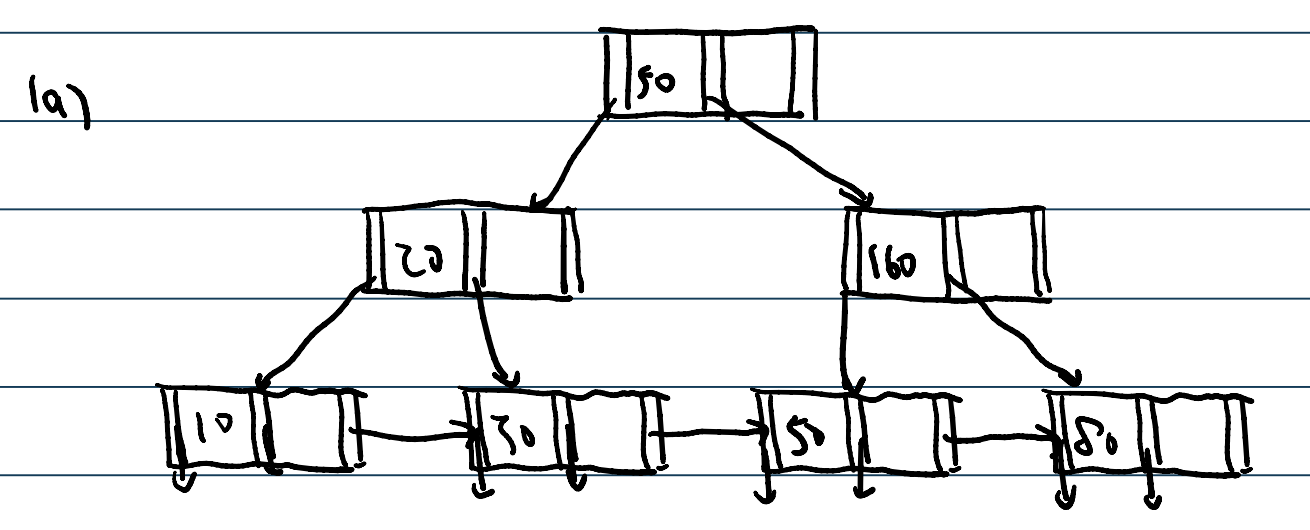
\includegraphics[width=5in]{1a.png}
                    \end{center}
              \item $ $
                    \begin{center}
                        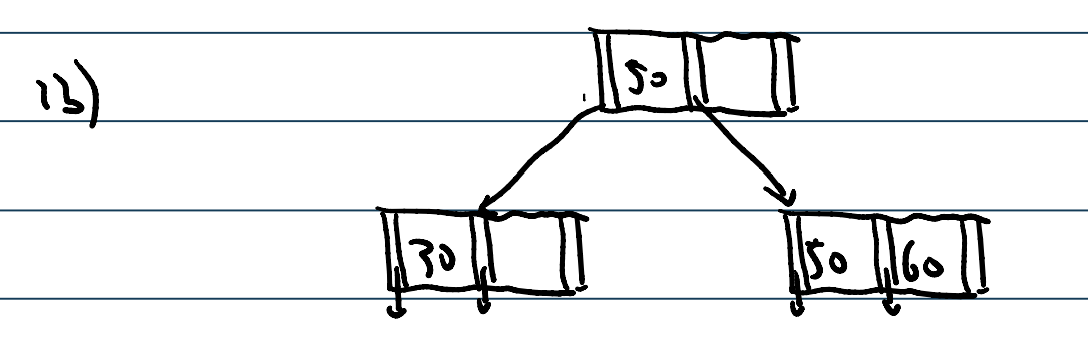
\includegraphics[width=5in]{1b.png}
                    \end{center}
          \end{enumerate}
    \item min: 8 ($\lceil\log_2(100)\rceil+1$), max: 100 (100 nodes of 3)
    \item $ $
    \begin{center}
        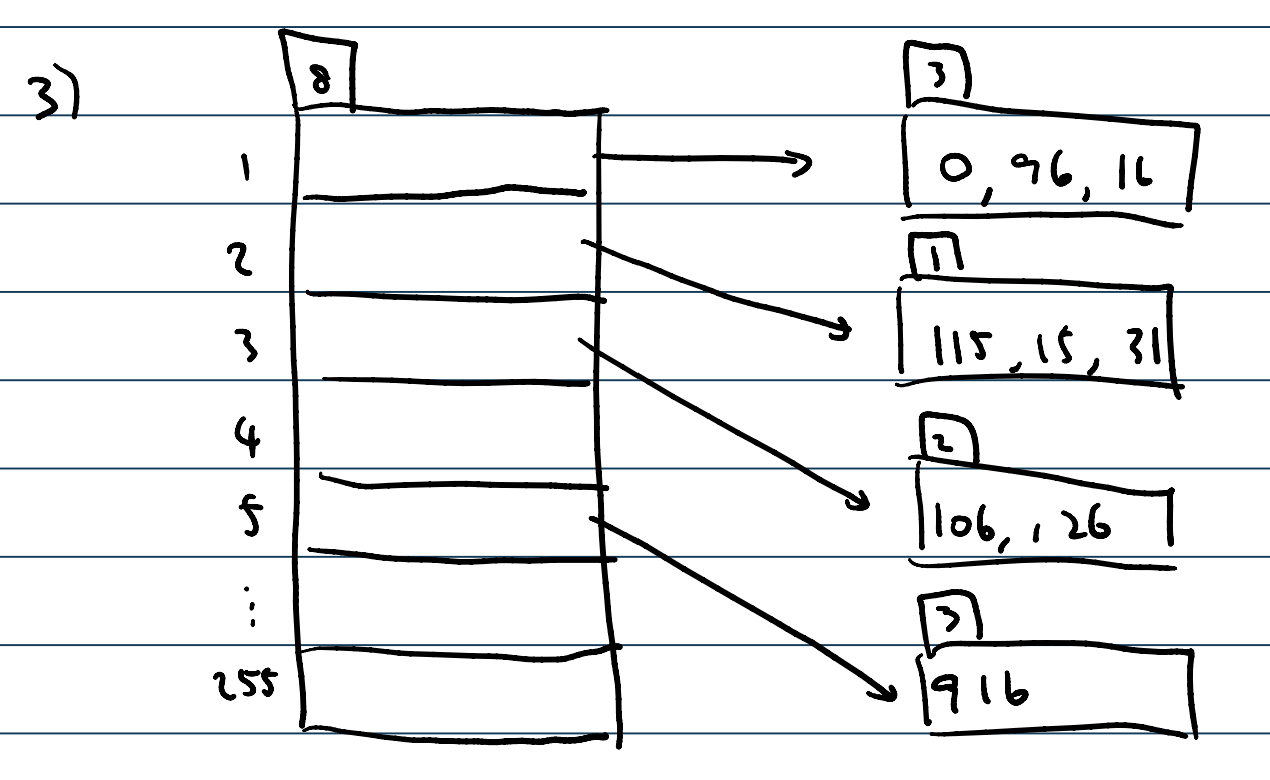
\includegraphics[width=5in]{3.png}
    \end{center}
\end{enumerate}
\end{document}